\chapter{Исследовательская часть}

\section{Технические характеристики}

Технические характеристики устройства, на котором выполнялось тестирование:

\begin{itemize}
	\item операционная система: Windows 10;
	\item оперативная память: 16 Гб;
	\item процессор: Intel® Core™ i5-8259U;
	\item количество ядер: 4;
	\item количество логических процессоров: 8.
\end{itemize}

Во время тестирования ноутбук был включен в сеть питания и нагружен только встроенными приложениями окружения и системой тестирования.

\section{Пример работы программы}
На рисунке \ref{fig:work_example} приведен пример работы программы.
\clearpage
\begin{figure}[h!]
	
	\centering{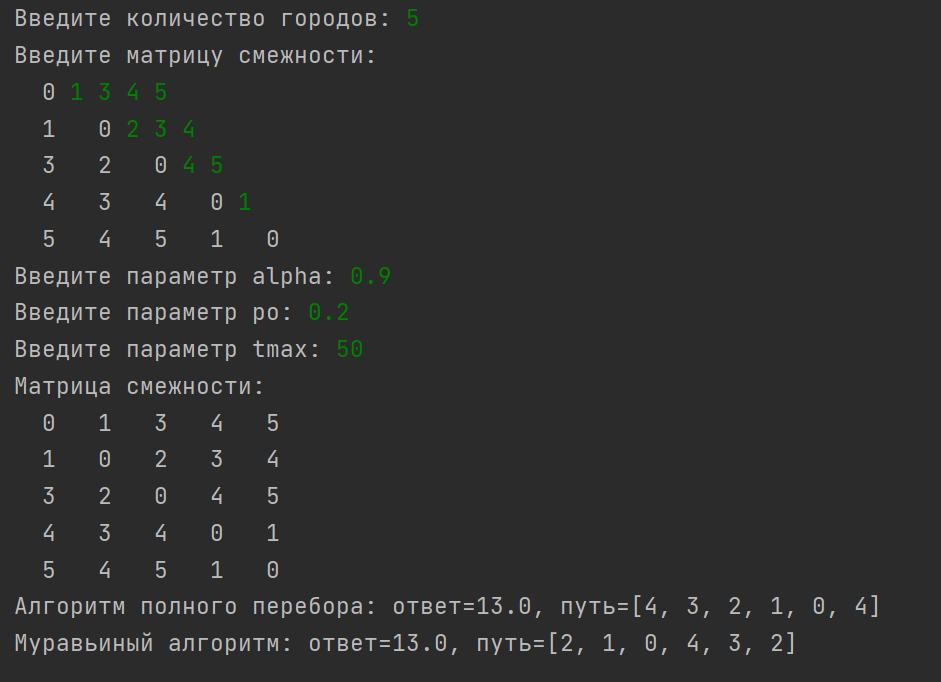
\includegraphics[scale=1]{inc/img/work_example.png}}
	
	\caption{Пример работы программы}
	
	\label{fig:work_example}
	
\end{figure}


\section{Параметризация муравьиного алгоритма}

В муравьином алгоритме вычисления проводятся с использованием таких настраиваемых парамтеров, как $\alpha$ (коэффициент жадности), po (коэффициент испарения феромона) и tmax (время жизни колонии). Проведем параметризацию этого алгоритма, то есть подберем такие наборы параметров, при которых алгоритм работает лучше всего, то есть находит решение, наиболее близкое к эталонному. Эталонным будем считать решение, найденное алгоритмом полного перебора. 

Чтобы не "подгонять" алгоритм под конкретные входные данные (матрицу смежности), необходимо проводить тестирование на нескольких классах данных. Возьмем три следующих класса: в первом и втором данные генерируются случайным образом, при этом разброс длин путей в первом (small) равен 10, во втором (big) - 1000, в третьем же классе (local) все длины путей задаются равными 12, затем прокладывается единственный оптимальный маршрут, в котором все города связаны путям длиной 8, а также специально создаются несколько локальных минимумов добавлением нескольких путей длины 10. Чтобы набор параметров претендовал на наилучший, алгоритм с такими настройками должен "хорошо" обработать каждый класс матриц смежности. 
 
Будем рассматривать матрицы размерности 11 × 11, чтобы получение точного результата муравьиным алгоритмом было более затруднено и сильнее зависело от параметров. Для параметров  $\alpha$ и po будем (независимо друг от друга) задавать значения [0.1, 0.25, 0.5, 0.75, 0.9], а для tmax - [100, 200, 300, 400, 500]. 

Результаты тестирования приведены на рисунках \ref{fig:tab1}-\ref{fig:tab5}, где $diff_x$ - разница между эталонным решением и решением, полученным с помощью муравьиного алгоритма на классе данных x, а diff\_sum - сумма всех разностей, поделенных на разброс длин путей в соответсвующем классе данных. Результаты отсортированы по возрастанию значений колонки diff\_sum. Вторым параметром сортировки стал tmax, так как при равном качестве алгоритм, использовавший меньшее число итераций, является более оптимальным.


\clearpage
\begin{figure}[h!]
	
	\centering{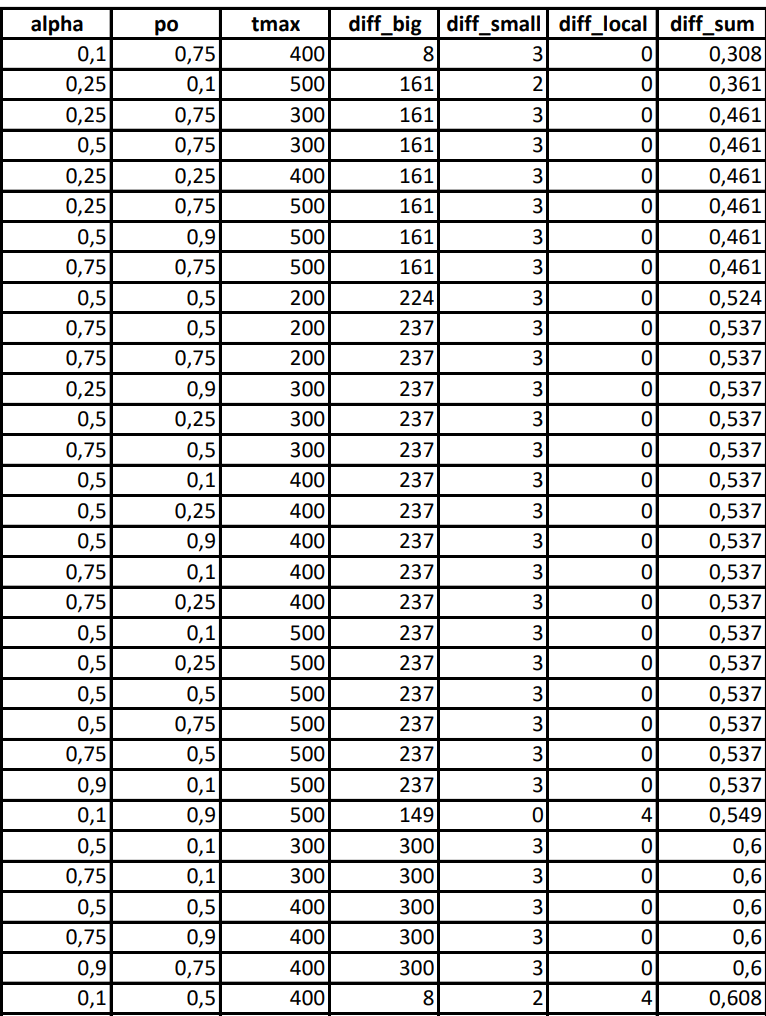
\includegraphics[scale=1]{inc/img/tab1.png}}
	
	\caption{Результаты параметризации, часть 1}
	
	\label{fig:tab1}
	
\end{figure}

\clearpage
\begin{figure}[h!]
	
	\centering{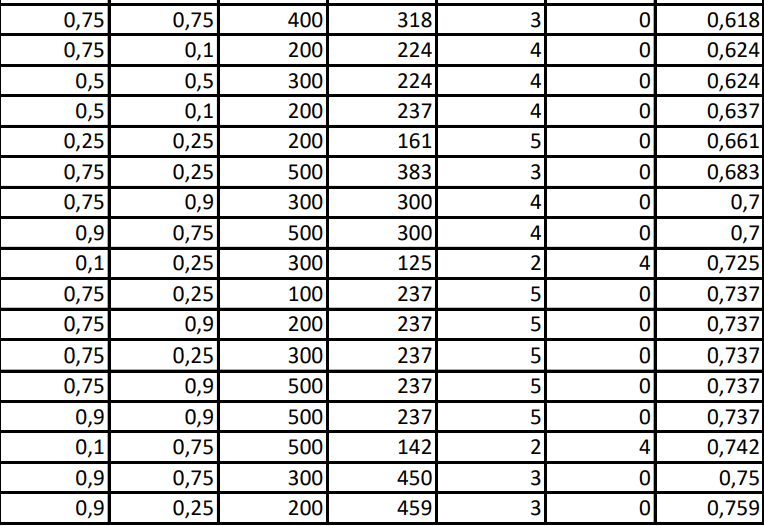
\includegraphics[scale=1]{inc/img/tab2.png}}
	
	\caption{Результаты параметризации, часть 2}
	
	\label{fig:tab2}
	
\end{figure}

\clearpage
\begin{figure}[h!]
	
	\centering{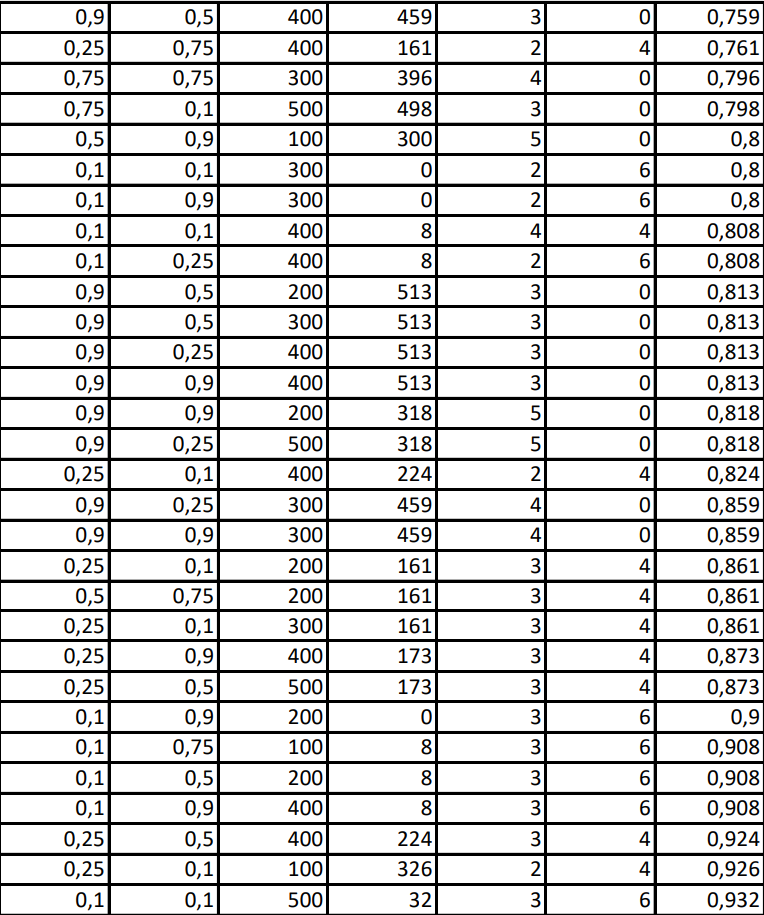
\includegraphics[scale=1]{inc/img/tab3.png}}
	
	\caption{Результаты параметризации, часть 3}
	
	\label{fig:tab3}
	
\end{figure}

\clearpage
\begin{figure}[h!]
	
	\centering{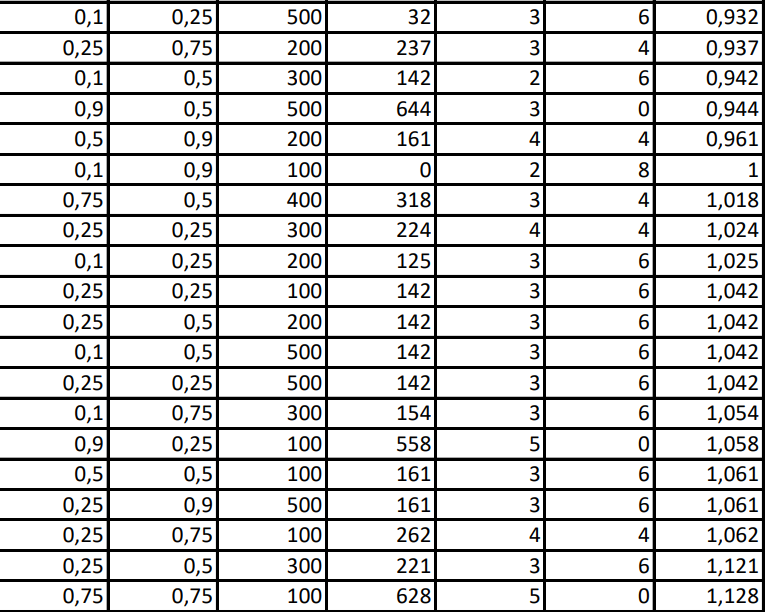
\includegraphics[scale=1]{inc/img/tab4.png}}
	
	\caption{Результаты параметризации, часть 4}
	
	\label{fig:tab4}
	
\end{figure}

\clearpage
\begin{figure}[h!]
	
	\centering{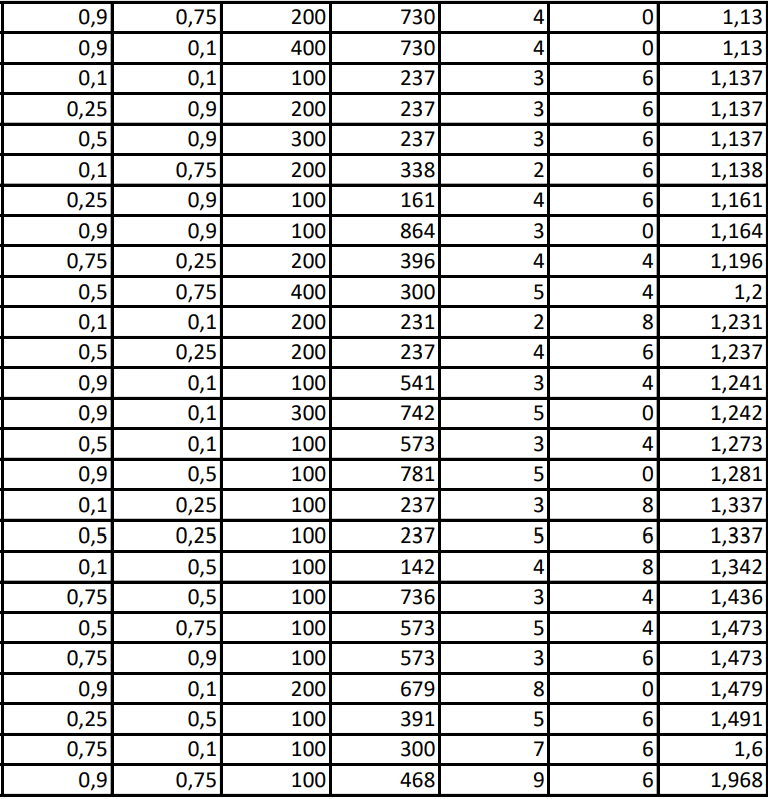
\includegraphics[scale=1]{inc/img/tab5.png}}
	
	\caption{Результаты параметризации, часть 5}
	
	\label{fig:tab5}
	
\end{figure}

Наилучшим образом на всех классах данных отработал муравьиный алгоритм с параметрами ($\alpha=0.1$, po=0.75 и tmax=400), за ним - с параметрами ($\alpha=0.25$, po=0.1 и tmax=500) и ($\alpha=0.25$, po=0.75 и tmax=300). При проведении таких же экспериментов для матриц меньшей размерности трудно определить 'параметры-победители', так как алгоритм в целом ошибается очень редко.

 В целом же по результатам параметризации можно сделать следующие выводы:
 \begin{enumerate}[label={\arabic*)}]
 	\item муравьиный алгоритм хорошо справляется с небольшими графами вне зависимости от параметров;
 	\item на матрицах достаточно большой размерности (в нашем примере - 11х11) он ошибается чаще и становится более зависимым от параметров;
 	\item на матрицах большой размерности при po=const и tmax=const меньшее значение $\alpha$, которое приближает алгоритм к жадности, приводит к лучшим результатам в сравнении с большими значениями;
 	\item при po=const и $\alpha$=const большее время жизни колонии tmax позволяет получить ответ более близкий к эталонному.
 \end{enumerate}
 


\section{Сравнение трудоемкостей реализаций}

Задача коммивояжера является NP-трудной, и точный переборный алгоритм ее решения имеет факториальную сложность. Сложность муравьиного алгоритма равна $O(tmax*m*n^2))$, то есть она зависит от времени жизни колонии, количества городов и количества муравьев в колонии.  ~\cite{first_article}. В данной реализации количество муравьев равно количеству городов, и трудоемкость муравьиного алгоритма равна $O(tmax * n^3)$.

\section{Сравнение времени выполнения реализаций алгоритмов}

Сравнивалось процессорное время работы алгоритма полного перебора и муравьиного алгоритма с параметрами, выбранными в результате параметрзации ($\alpha=0.1$, po=0.75 и tmax=400). Эти реализации сравнивались по времени работы при количестве городов от 3 до 11 с шагом 1.
 
Так как некоторые задачи выполняются достаточно быстро, а замеры времени имеют некоторую погрешность, они для каждой реализации и каждого количества заявок выполнялись 10 раз, а затем вычислялось среднее время работы.
 

На рисунке \ref{img:time_all} приведены результаты сравнения времени выполнения реализаций алгоритмов. 

\clearpage
\img{120mm}{time_all}{Сравнение времени работы реализаций в зависимости от количества городов}

Как видно из графиков, теоретическая оценка трудоемкости подтвердилась: время работы алгоритма полного перебора растет как O(n!), а муравьиного алгоритма - как O($n^3$), где n - количество городов. В связи с этим при небольшом количестве городов (до 8 включительно) алгоритм полного перебора находит решение за меньшее количество времени по сравнению с муравьиным алгоритмом, однако далее с ростом числа городов начинает все стремительней уступать второму.


\section{Вывод из исследовательской части}

Таким образом, в ситуациях, когда количество городов велико (более 8, например), а задача коммивояжера не требует абсолютно точного ответа, для ее решения можно использовать муравьиный алгоритм вместо алгоритма полного перебора, что позволит сэкономить процессорное время. При этом заранее проведенная параметризация может помочь настроить первый алгоритм так, что и он будет в большинстве случаев выдавать точный ответ. 

При небольшом же размере графа (прмерно до размерности 8х8) муравьиный алгоритм с большой вероятностью даст точный ответ, однако в этом случае он не дает выигрыша по времени перед алгортмом полного перебора.